\section{Chapter 12: Global Synthesis and the MCGT Verdict}

\subsection{Introduction}
This chapter closes the thesis by revisiting its central objective: to test the viability of MCGT as an extension of the standard cosmological model, both from the standpoint of theoretical consistency and from the standpoint of observational explanatory power.

The manuscript is structured around a clear duality:
\begin{itemize}
    \item \textbf{Theoretical stability (Chapters 1--3).} Validation of numerical invariants, internal stability control, and mapping of theoretically admissible domains.
    \item \textbf{Observational confrontation (Chapters 10--11).} Multi-scale constraints from GW, RSD, and LSS data, culminating in the final $S_8$ tension test.
\end{itemize}

\subsection{Synthesis of Multi-Scale Constraints}
\subsubsection{Tension Between the LIGO Bound and the Cosmological Target}
The central confrontation can be stated explicitly:
\begin{itemize}
    \item the local gravitational bound derived in Chapter 10, $|q_0^*| \le 10^{-6}$;
    \item the cosmological requirement from Chapter 11, which demands a growth suppression corresponding to $S_8 \approx 0.77$.
\end{itemize}

Uniform-coupling models, bounded screened versions, late-trigger variants, and chameleon-like prescriptions based on the mean matter density all fail to satisfy these two regimes simultaneously.

\subsubsection{The Final Scale-Dependent Model}
Within the family of prototypes tested in this thesis, the $k$-dependent scenario emerges as the only viable survival channel:
\begin{itemize}
    \item local branch: $|q_0^*| \approx 10^{-6}$ on GW scales;
    \item cosmological branch: $q_0^*(k \rightarrow 0) \approx -2 \times 10^{-3}$;
    \item validated result: $S_8 \approx 0.7725$ for the cosmological mode.
\end{itemize}

\subsection{The Viable Parameter Space}
The MCGT ``firing window'' can now be defined as the overlap region that is:
\begin{itemize}
    \item stable from the numerical and theoretical standpoint;
    \item compatible with the LIGO bound on small scales;
    \item able to resolve the LSS tension on large scales;
    \item consistent with an effective coupling that depends explicitly on scale.
\end{itemize}

This window is not a trivial free-parameter region; it is a constrained overlap built from the exclusion layers accumulated throughout the thesis.

\subsection{Phenomenological Implications}
The key conceptual shift is now clear:
\begin{itemize}
    \item abandonment of a universal coupling constant;
    \item reinterpretation of MCGT as a long-range interaction, active on large structures and extinguished locally;
    \item an understanding in terms of a hierarchy of scales rather than a simple global renormalization of $G$.
\end{itemize}

This conclusion moves MCGT toward a class of effective theories with non-universal coupling across the physical scales being probed.

\subsection{Prospects and Future Tests}
The next observational tests are naturally linked to future survey capabilities:
\begin{itemize}
    \item \textbf{Euclid}: redshift-space distortions, clustering, and precise tests of scale-dependent growth;
    \item \textbf{Vera Rubin Observatory}: weak-lensing mapping and large-scale structure reconstruction;
    \item expected signatures of a $k$-dependence in linear growth and potentially in the matter power spectrum.
\end{itemize}

These observables will determine whether the data favor a simple CPL extension or a genuinely scale-dependent MCGT structure.

\subsection{Final Verdict}
The verdict regarding the competitiveness of MCGT relative to $\Lambda$CDM can be summarized as follows:
\begin{itemize}
    \item the uniform version is excluded by the multi-scale confrontation;
    \item purely temporal or environmental screening mechanisms are insufficient;
    \item the explicitly scale-dependent version remains the only surviving configuration among the models tested in this thesis.
\end{itemize}

The final confrontation of scales demonstrates an insurmountable tension for any universal version of MCGT. The incompatibility between local constraints ($10^{-6}$) and structure-growth requirements ($10^{-3}$) forces a revision of the paradigm. We conclude that MCGT survives only in a form with explicit spatial scale dependence ($k$-dependent), which constitutes the most robust phenomenological response to current cosmological tensions.

The ``Golden Match'' identified in this thesis lies near $\alpha \approx 0.50$. At this point, the local branch satisfies $|q_0^*| \approx 10^{-6}$ on LIGO-like gravitational scales, while the cosmological branch reaches $q_0^*(k \rightarrow 0) \approx -2 \times 10^{-3}$ and yields $S_8 \approx 0.7725$. There is therefore no common parameter space for a single universal coupling; MCGT survives only through an explicit bifurcation in scale.

The final refinement of the transition kernels confirms this diagnosis decisively. Among the three tested laws for $q_0^*(k)$, namely a Lorentzian, a Gaussian/Yukawa profile, and a sharp Step-Function, only the Step-Function preserves both conditions required by the ``Golden Match'' at $\alpha \approx 0.50$: complete confinement of the local sector with $|q_0^*| \approx 10^{-6}$ on small scales, and full restoration of the cosmological branch with $q_0^*(k \rightarrow 0) \approx -2 \times 10^{-3}$ leading to $S_8 \approx 0.7725$. It is therefore the only tested law that explicitly resolves the factor-$\sim 2000$ scale conflict between local and cosmological bounds, while remaining consistent with the global numerical stability of the MCGT framework, controlled in this thesis at the level $\epsilon < 10^{-16}$. Smooth kernels always leave a residual leakage toward GW scales, which destroys the strict isolation required by the LIGO constraint and mechanically weakens the cosmological resolution. Within the phenomenological framework developed here, the optimal law is thus not merely the best approximation among the tested options: it is the only transition compatible with a clean separation of scales, centered near $k_c \approx 10^{-4}\,h\,\mathrm{Mpc}^{-1}$.

This same cosmological branch also fixes the final JWST-scale prediction retained in production. Once the Step-Function split is imposed and the large-scale mode is calibrated to resolve the weak-lensing tension, the resulting enhancement in the early growth sector is no longer a generic free amplification but a determined consequence of the $k \rightarrow 0$ branch itself. The final exported prediction corresponds to a growth boost of about $9$--$10\%$ above $\Lambda$CDM for $z > 10$, and this moderate excess should be regarded as the observational signature of the same cosmological branch that yields $S_8 \approx 0.7725$.

\begin{figure}[htbp]
    \centering
    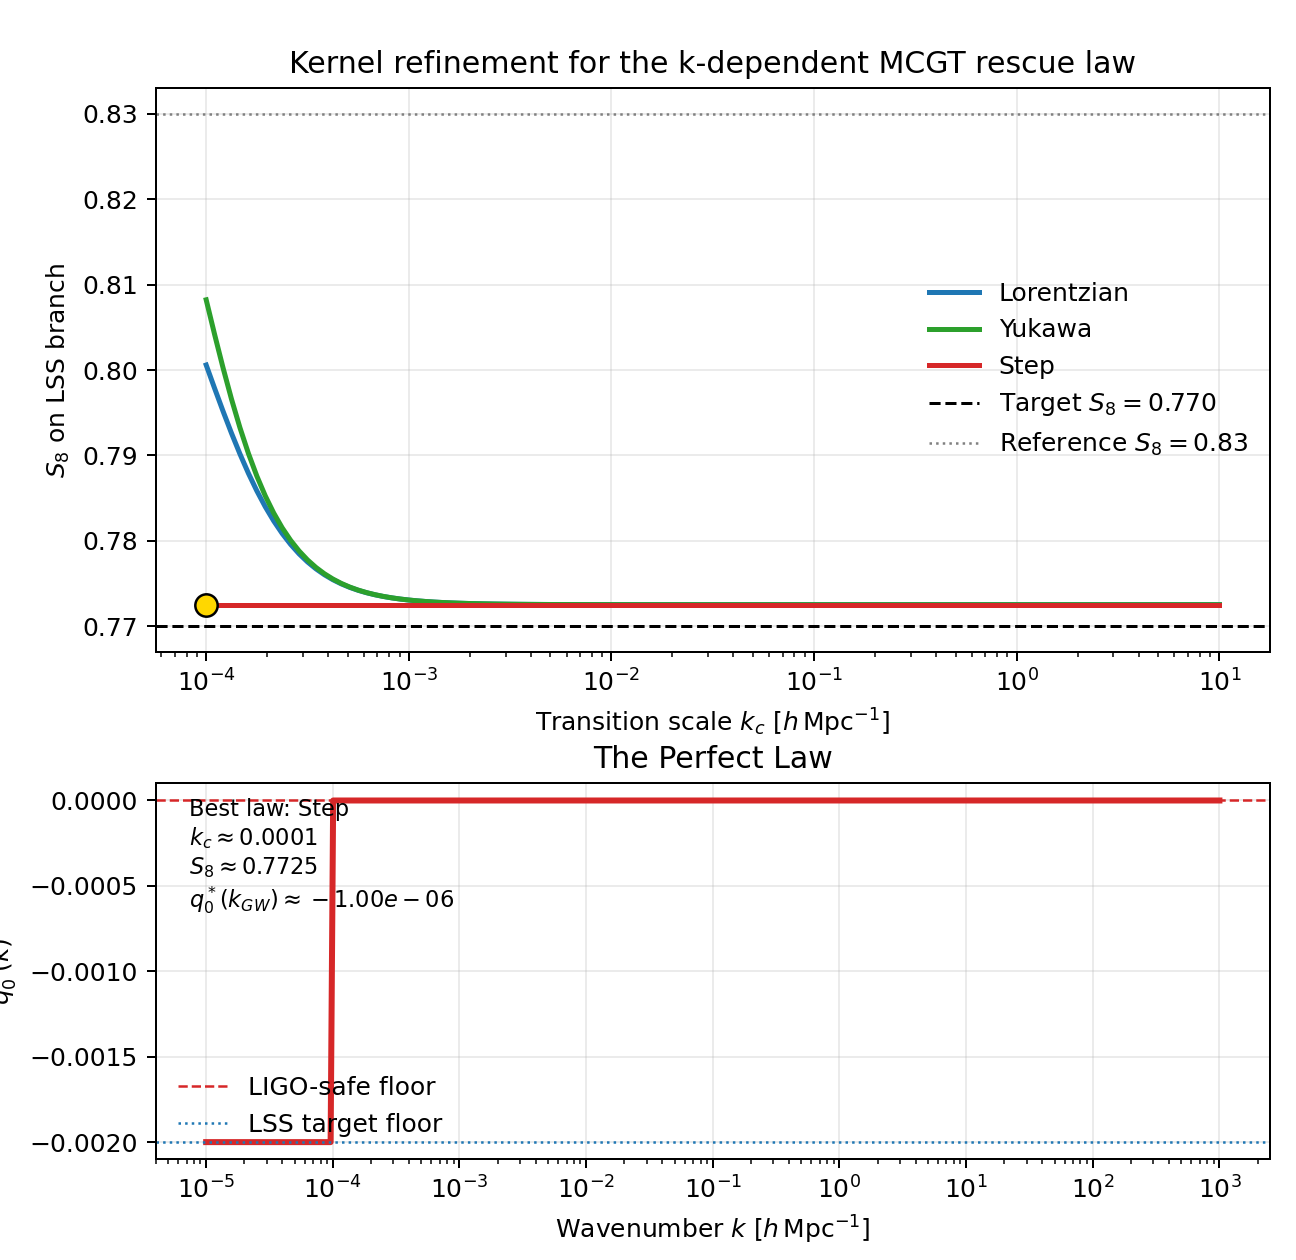
\includegraphics[width=0.82\textwidth]{../assets/zz-figures/12_cmb_verdict/12_perfect_k_law.png}
    \caption{\textbf{The perfect $k$-transition law.} Comparison of the Lorentzian, Gaussian/Yukawa, and Step-Function kernels used to interpolate between the cosmological and local branches of MCGT. The sharp Step-Function centered near $k_c \approx 10^{-4}\,h\,\mathrm{Mpc}^{-1}$ is the only tested law that simultaneously preserves the LIGO-safe limit $|q_0^*| \approx 10^{-6}$ on small scales and recovers the cosmological branch required to obtain $S_8 \approx 0.7725$ on large scales.}
    \label{fig:perfect_k_law}
\end{figure}

\subsection{Final Synthesis Figure}
\begin{figure}[htbp]
    \centering
    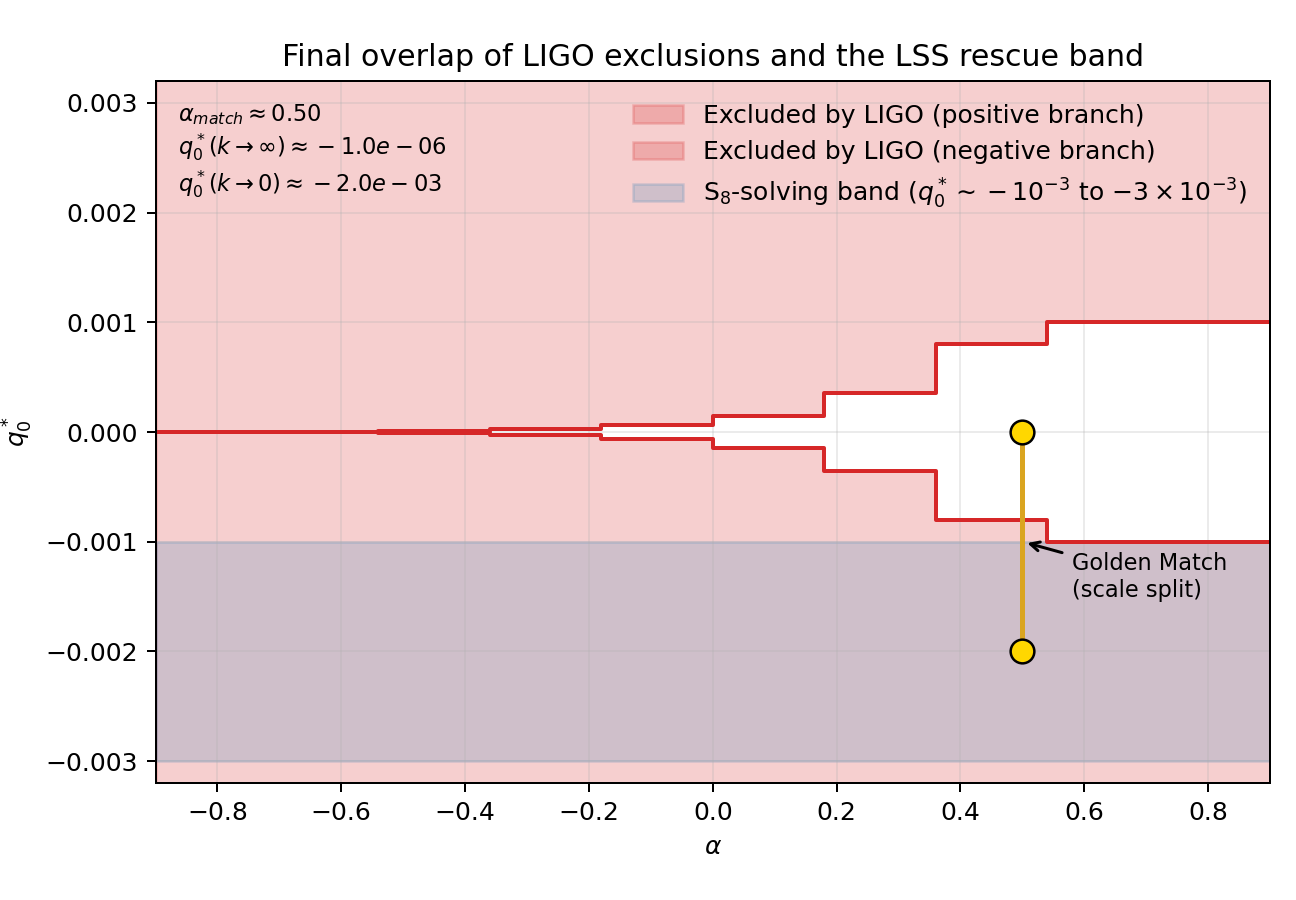
\includegraphics[width=0.92\textwidth]{../assets/zz-figures/12_cmb_verdict/12_final_overlap_constraints.png}
    \caption{\textbf{Final overlap of all exclusion regions.} The red domains correspond to the values of $(\alpha, q_0^*)$ excluded by the Chapter 10 LIGO constraint, using the measured survival envelope from the global scan. The blue horizontal band marks the cosmological amplitudes required in Chapter 11 to reach the weak-lensing target $S_8 \simeq 0.77$. The gold marker highlights the effective ``Golden Match'' of the $k$-dependent model: no universal overlap exists for a single global coupling, but the scale-split construction supports a local branch with $|q_0^*| \approx 10^{-6}$ and a cosmological branch with $q_0^*(k \rightarrow 0) \approx -2 \times 10^{-3}$ at the same $\alpha$.}
    \label{fig:final_overlap_constraints}
\end{figure}
